\lstset{language=Java, numbers=left, numberstyle=\tiny, stepnumber=2, numbersep=5pt}
\chapter{Introduction}
\label{intro}
As the last few years and decades have seen ever-increasing amounts of data analyzed and managed in ever shorter periods of time, a challenge faced by the IT industry has been the limited computing power of individual machines and simple networks. Tasks are constantly evolving, so they need more and more computing power to solve them.\\
In order to solve these problems, various techniques have been developed that help to continuously improve the performance of the machines. These include supercomputers, computer clusters, and various methods and algorithms that can be summarized under the term High Performance Computing.\\
This workshop introduces the programming model \textbf{MapReduce} and a simulation of the model based on the \textbf{Hadoop} framework. The aim of this workshop was to use the Hadoop Simulation HSim to gain a basic understanding of the functionality of MapReduce.
%%%%%%%%%%%%%%%%%%%%%%%%%%%%%%%%%%%%%%%%%%%%%%%%%%%%%%%%%%%%%%%%%%%%%%%%%%%%%%%%%%%%%%%%%%%%%%%%%%%%%%%%%
%%%%%%%%%%%%%%%%%%%%%%%%%%%%%%%%%%%%%%%%%%%%%%%%%%%%%%%%%%%%%%%%%%%%%%%%%%%%%%%%%%%%%%%%%%%%%%%%%%%%%%%%%
%%%%%%%%%%%%%%%%%%%%%%%%%%%%%%%%%%%%%%%%%%%%%%%%%%%%%%%%%%%%%%%%%%%%%%%%%%%%%%%%%%%%%%%%%%%%%%%%%%%%%%%%%
\chapter{High Performance Computing With MapReduce and Hadoop}
\label{mapreduce}
As already mentioned in the introduction, MapReduce was introduced as a programming model to process large amounts of data (Big Data) in parallel on several machines. This reduces processing time, since the load can be distributed over multiple machines.\\
The following chapters briefly explain the basics of this workshop. First, MapReduce and its functionality are described. This is followed by a short introduction to Hadoop.
\subsection{MapReduce}
\begin{figure}[H]
	\centering
	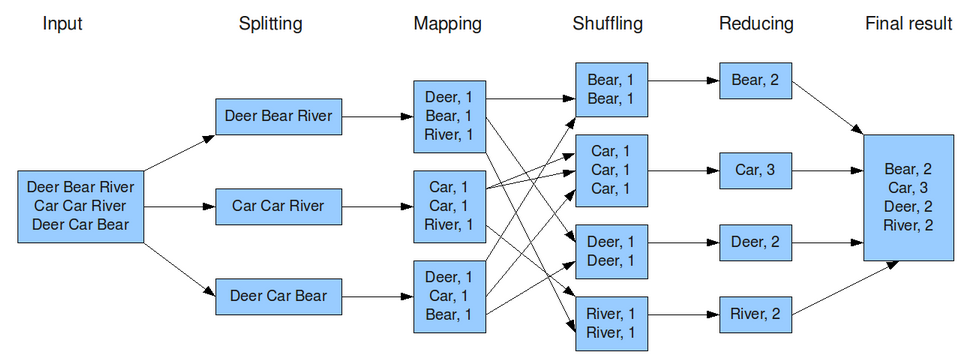
\includegraphics[width=1.0\linewidth]{mapreduce.PNG}
	\caption[Caption for LOF]{The MapReduce model\footnotemark}
	\label{mapreducepic}
\end{figure}
\footnotetext{image-source: https://cs.calvin.edu/courses/cs/374/exercises/12/lab}

\subsection{Hadoop}
\cite[see][]{AP1}
%%%%%%%%%%%%%%%%%%%%%%%%%%%%%%%%%%%%%%%%%%%%%%%%%%%%%%%%%%%%%%%%%%%%%%%%%%%%%%%%%%%%%%%%%%%%%%%%%%%%%%%%%
%%%%%%%%%%%%%%%%%%%%%%%%%%%%%%%%%%%%%%%%%%%%%%%%%%%%%%%%%%%%%%%%%%%%%%%%%%%%%%%%%%%%%%%%%%%%%%%%%%%%%%%%%
%%%%%%%%%%%%%%%%%%%%%%%%%%%%%%%%%%%%%%%%%%%%%%%%%%%%%%%%%%%%%%%%%%%%%%%%%%%%%%%%%%%%%%%%%%%%%%%%%%%%%%%%%
\chapter{Hadoop's Parameters}
\label{params}

%%%%%%%%%%%%%%%%%%%%%%%%%%%%%%%%%%%%%%%%%%%%%%%%%%%%%%%%%%%%%%%%%%%%%%%%%%%%%%%%%%%%%%%%%%%%%%%%%%%%%%%%%
%%%%%%%%%%%%%%%%%%%%%%%%%%%%%%%%%%%%%%%%%%%%%%%%%%%%%%%%%%%%%%%%%%%%%%%%%%%%%%%%%%%%%%%%%%%%%%%%%%%%%%%%%
%%%%%%%%%%%%%%%%%%%%%%%%%%%%%%%%%%%%%%%%%%%%%%%%%%%%%%%%%%%%%%%%%%%%%%%%%%%%%%%%%%%%%%%%%%%%%%%%%%%%%%%%%
\chapter{HSim}
\label{hsim}
As already mentioned in the introduction, no complete cluster is being set up for this workshop, as the effort would have been far too much. Instead the provided software \textit{HSim} was used, which provides a simulated Hadoop environment with several machines, routers and nodes. HSim and is based on Java and Hadoop v2 and it offers the possibility to adjust different Hadoop parameters and to display the effects on the simulation realistically.
%%%%%%%%%%%%%%%%%%%%%%%%%%%%%%%%%%%%%%%%%%%%%%%%%%%%%%%%%%%%%%%%%%%%%%%%%%%%%%%%%%%%%%%%%%%%%%%%%%%%%%%%%
%%%%%%%%%%%%%%%%%%%%%%%%%%%%%%%%%%%%%%%%%%%%%%%%%%%%%%%%%%%%%%%%%%%%%%%%%%%%%%%%%%%%%%%%%%%%%%%%%%%%%%%%%
%%%%%%%%%%%%%%%%%%%%%%%%%%%%%%%%%%%%%%%%%%%%%%%%%%%%%%%%%%%%%%%%%%%%%%%%%%%%%%%%%%%%%%%%%%%%%%%%%%%%%%%%%
\chapter{Evaluation}
\label{eval}
\subsection{Changing the dataSize}
\subsection{Changing the sortFactor}
\subsection{Changing the requiredMappers and requiredReducers}

%%%%%%%%%%%%%%%%%%%%%%%%%%%%%%%%%%%%%%%%%%%%%%%%%%%%%%%%%%%%%%%%%%%%%%%%%%%%%%%%%%%%%%%%%%%%%%%%%%%%%%%%%
%%%%%%%%%%%%%%%%%%%%%%%%%%%%%%%%%%%%%%%%%%%%%%%%%%%%%%%%%%%%%%%%%%%%%%%%%%%%%%%%%%%%%%%%%%%%%%%%%%%%%%%%%
%%%%%%%%%%%%%%%%%%%%%%%%%%%%%%%%%%%%%%%%%%%%%%%%%%%%%%%%%%%%%%%%%%%%%%%%%%%%%%%%%%%%%%%%%%%%%%%%%%%%%%%%%
\chapter{Conclusion}
\label{conlusion}


